\chapter{Basics of Word2Vec Model and Echo State Network}\label{basics}

This chapter establishes the background knowledge required for this research work. The chapter is divided into two section. In the first section, the basics of Word2Vec model, the flavors in which the model exist, the training of the Word2Vec model and the properties of the word embeddings learned by the model. In the second section, the basics of Echo State Network and how it is trained is described. 

\section{Word2Vec Model}

Word2Vec model is a neural probabilistic language model proposed by Mikolov et al. \cite{w2v:mikolov_2013_distributed}. The model is based on the distributional hypothesis which states that the words that appear in the same context share the semantic meaning \cite{w2v:tensor_flow}. The main idea behind the model is to learn the word embeddings from the context words (nearby words). The model takes a large text data, to generate the distributed embeddings of the words present in the text and also preserves the linear regularities among words. In other words, it maps the words into a continuous vector space where semantically related words are placed close to each other. Earlier the words have been treated as discrete atomic symbols in all traditional \acs{NLP} systems where the words are represented in a localist fashion. Localist representation of words does not contain any semantic or syntactic information about the word and thus depriving the \acs{NLP} systems to utilize this information while processing \cite{w2v:baroni:2014}. Word2Vec neural word embeddings overcome this issue and capture the semantics and syntactic information of the word in a computationally-efficient manner \cite{w2v:mikolov_2013_efficient}. For learning the word embeddings, the Word2Vec model exists in two neural architectures, the \ac{CBOW} and \ac{SG} \cite{w2v:mikolov_2013_efficient, w2v:mikolov_2013_distributed}. Figure \ref{fig:cbow} and \ref{fig:sg} shows the neural architecture of \acs{CBOW} and \acs{SG} models respectively. Both the CBOW and SG model have three neural layers, i.e., an input layer, a hidden layer and an output layer. Although, both the models are architecturally similar but have different training objectives. The next sections, provide a brief overview of \acs{CBOW} model and \acs{SG} model. However, in this work skip-gram model will be used because it was shown that it generate better word-embeddings as compared to CBOW \cite{w2v:mikolov_2013_distributed}.

\subsection{CBOW model}

\begin{figure}[hbtp]
\centering
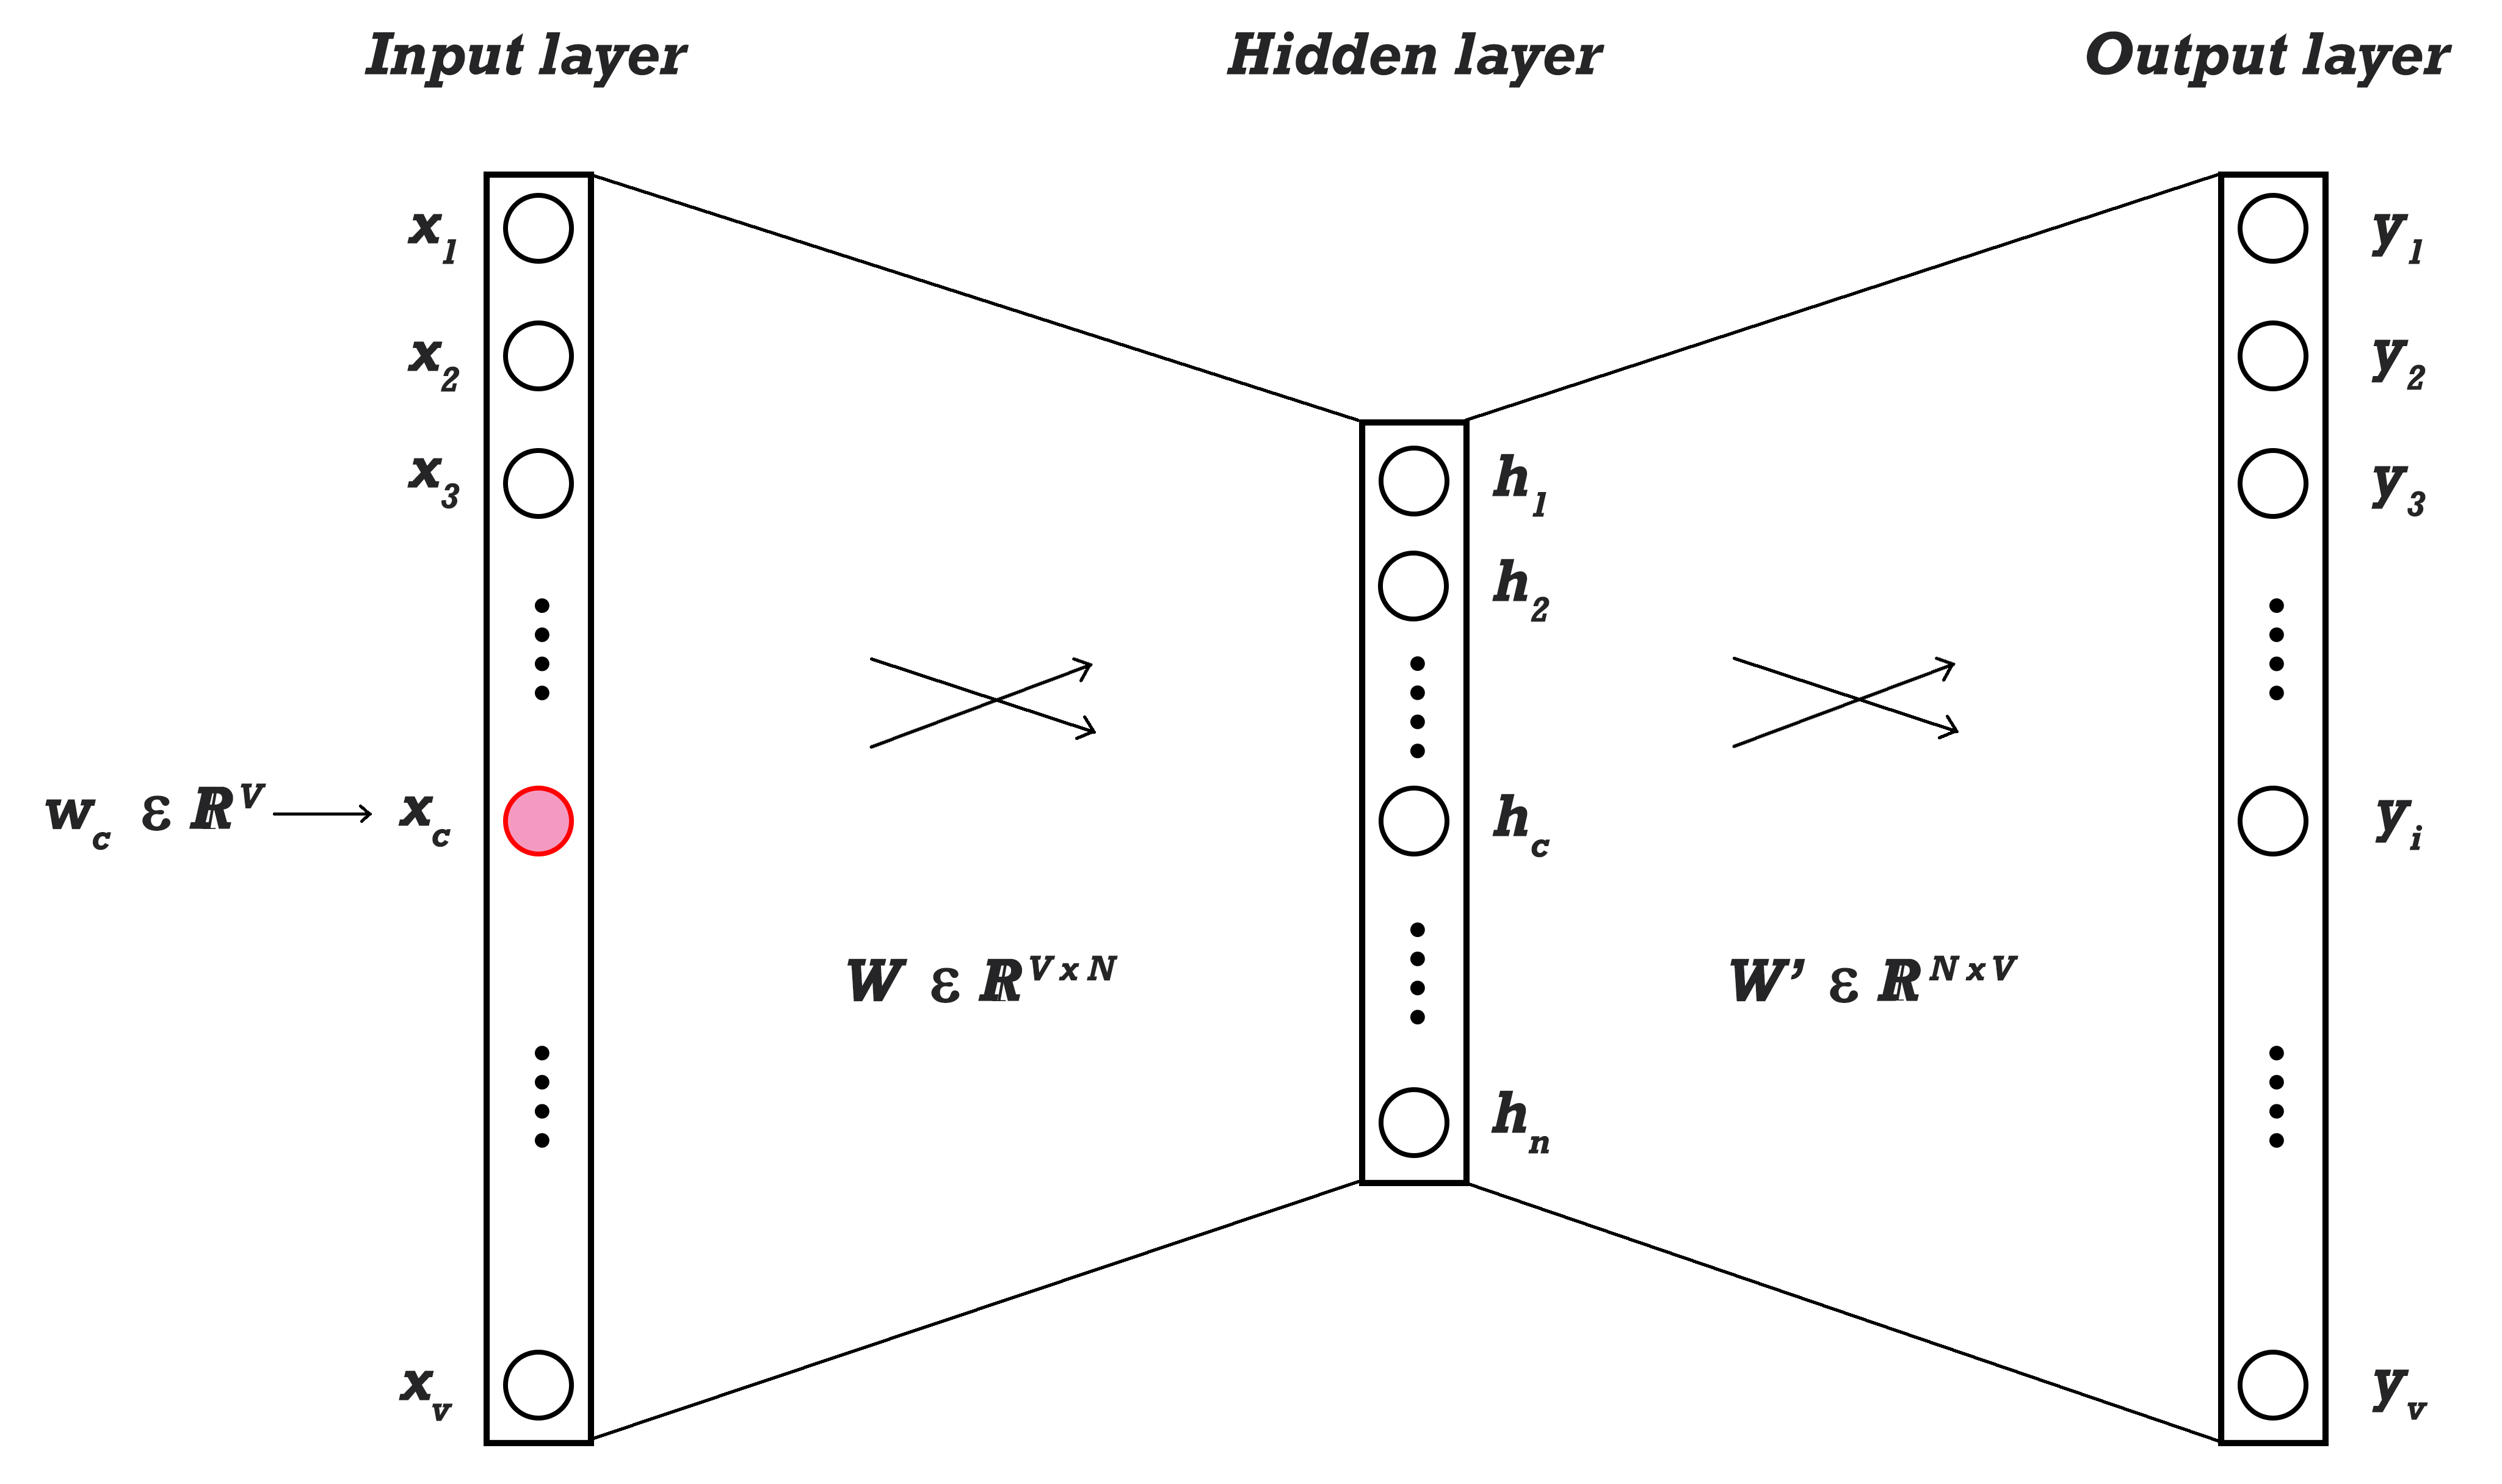
\includegraphics[width=0.8\linewidth,height=10cm,keepaspectratio]{cbow}
\caption[The CBOW model.]{\textbf{The CBOW model: }{\small The objective of CBOW model is to predict the target word based on the context words (or neighboring words). Given a vocabulary V, and desired vector dimension N, the context words are input to the model (in this case only one, $w_{c}$) using localist representation. Only one vector element corresponding to the input word is one ($x_{c}$, shown in red) and all other elements are 0. The model outputs the probability for each word in vocabulary, which is then maximized for the actual target word during training. Adapted from \cite{w2v:parameter_learning}.}}
\label{fig:cbow}
\end{figure}

CBOW  model is a three layered neural model with the training objective to predict a target word (e.g. Peter) given some context words (``John gave the ball to --"). Figure \ref{fig:cbow} shows the CBOW network architecture with a simplified case of one context word. The model is trained on the dataset having a vocabulary size $V$ in an unsupervised way to achieve the objective. The hidden layer is of size $N$; the dimensions of the desired word embeddings. The neurons in both the adjacent layers i.e. input and output layer are fully connected to the hidden layer neurons. The input to the network is the context word $w_c {\in} \mathbb{R}^{V}$ and is represented using localist representation, $w_c=[{x_1,..,x_c,..,x_V}]$ where only one unit $x_c$ at index c will be 1 out of V units and all other units will be 0 \cite{w2v:parameter_learning}. The activation of the hidden layer is then given by:

\begin{equation}\label{eqn:hidden_act}
    h = W^T . w_c= W_{(c,:)}=v_{c}
\end{equation}

\noindent where $W {\in} \mathbb{R}^{V{\times}N}$ is the weight matrix from input to hidden layer and $v_{c}$ is the vector embedding of the context word $w_c$. Equation \ref{eqn:hidden_act} basically copies the $c^{th}$ row of weight matrix $W$ on the hidden layer as the hidden layer activation function is linear. 

A score $u {\in}\mathbb{R}^V$ is then calculated for all the target words in the vocabulary, which is essentially the compatibility of a word $w_i$ given the context word $w_c$ \cite{w2v:parameter_learning}.

\begin{equation}
\begin{split}
         u &={W^{'}} ^ T . h \\
              &= {W^{'}}^T. v_{c}    
\end{split}
\end{equation}
\begin{equation}
    u_i = {W^{'}_i}^T. v_{c}
\end{equation}

\noindent where $u_i$ gives the score of $i^{th}$ word, $w_{i}$, for i = 1, 2,...,V. $W^{'}{\in} \mathbb{R}^{N{\times}V} $ is the weight matrix between hidden and output layer. ${W^{'}_i}$ is the $i^{th}$ column vector of matrix $W^{'}$.  
The computed scores are then converted to posterior probabilities by the output neurons with softmax activation function \cite{w2v:parameter_learning}. Thus aliasing ${W^{'}_i}$ as $v^{'}_{i}$, we get output probabilities as: 

\begin{equation}
\begin{split}    
y_i &= P(w_i | w_c) = \frac {\exp(u_i)} {\sum_{i' {\in} V} \exp (u_{i^{'}})}\\
    &= \frac {\exp({v^{'}_{i}}^T.v_{c})}{\sum_{i' {\in} V}\exp({v^{'}_{i^{'}}}^T.v_{c})}
\end{split}
\end{equation}

\noindent where $y_i$ is the probability of $i^{th}$ word ($w_{i}$) given the context word ($w_{c}$). The training objective is then achieved by maximizing the log likelihood of the actual target word $(w_{t})$ given the context word ($w_{c}$)   \cite{w2v:parameter_learning}. So the cost functions can be written as:

\begin{equation}
  \begin{split}
      J_{ML} &= max\ \log P(w_t | w_c) \\
           &= max\ {v^{'}_{t}}^T.v_{c}- \text{ log} \sum_{i' {\in} V} {\exp({v^{'}_{i^{'}}}^T.v_{c})}
  \end{split}
\end{equation} 

In the case, when multiple context words are input to the network, only the equation \ref{eqn:hidden_act} changes to:

\begin{equation}
h= \frac {1}{K} .(v_{c_1}+v_{c_2}+.......+v_{c_K}) 
\end{equation}    

\noindent where $k$ is the size of the context window. This equation averages the vector embeddings of all the context words \cite{w2v:parameter_learning}.

\subsection{Skip-gram model}

\begin{figure}[hbtp]
\centering
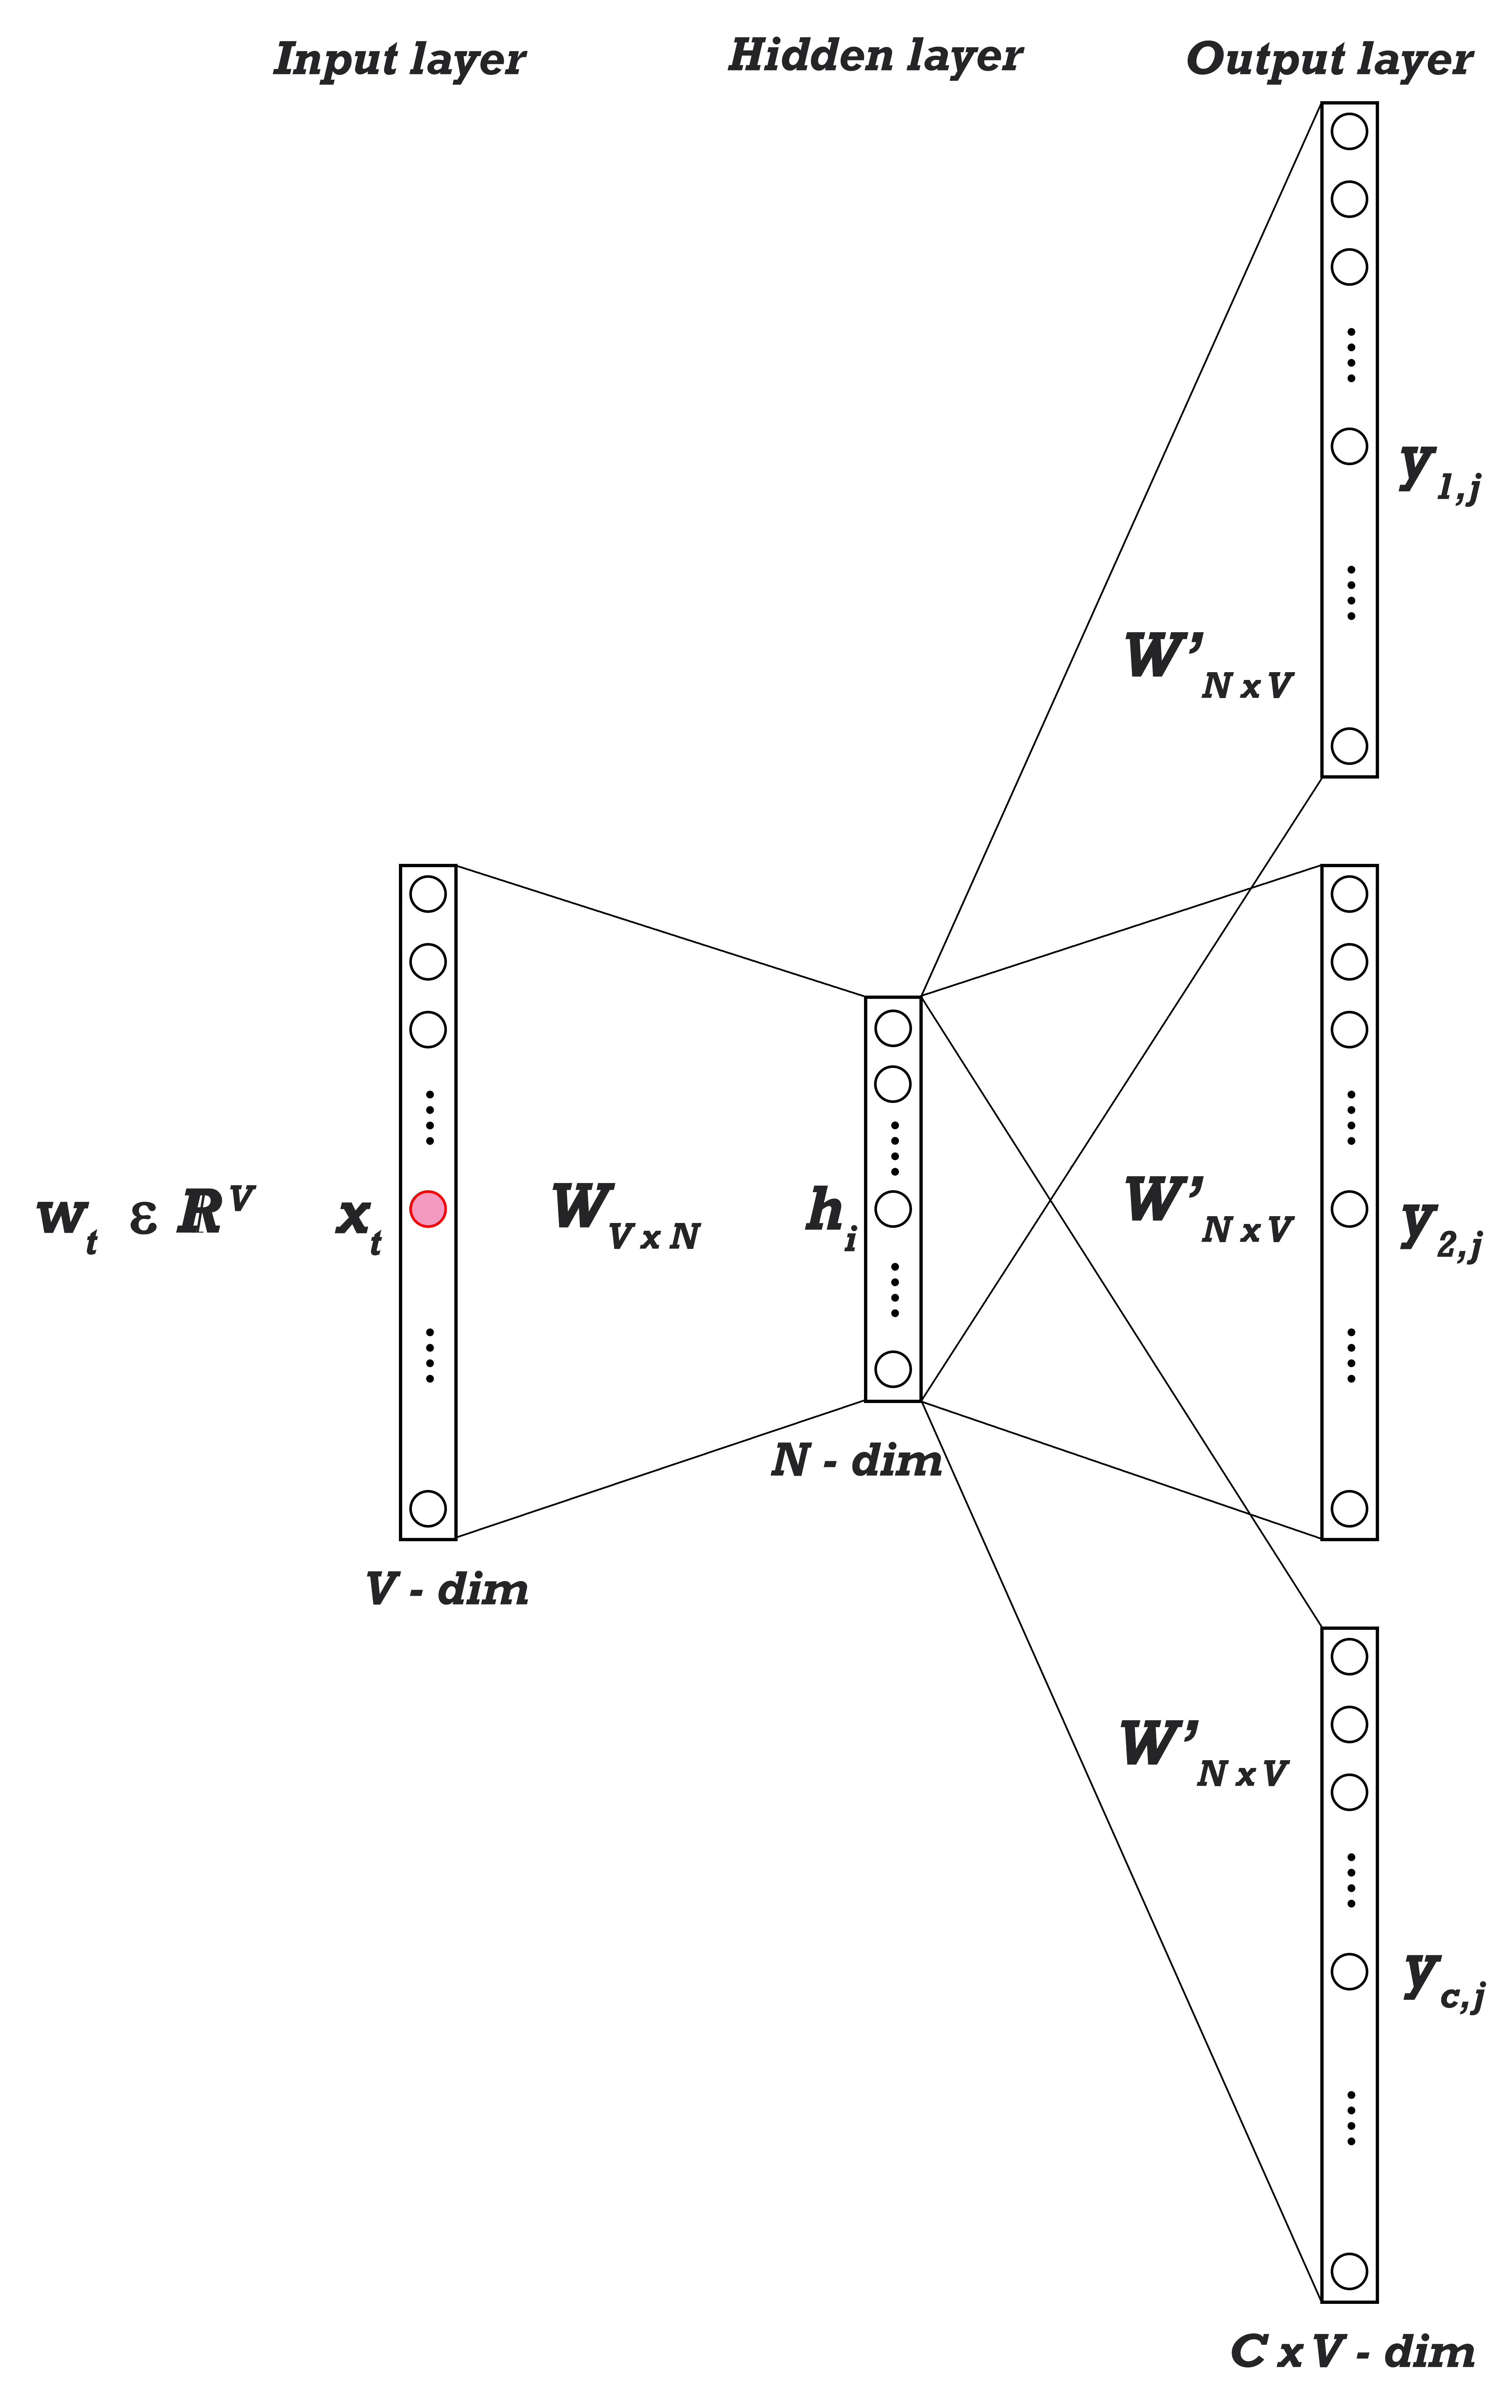
\includegraphics[width=1.8\linewidth,height=10cm,keepaspectratio]{sg}
\caption[The Skip-gram model.]{\textbf{The skip-gram model: }{\small The objective of Skip-gram model is the reverse of CBOW. It predicts the context words from a target word. Given a vocabulary V, and desired vector dimension N, The target word ($w_{t}$) is input to the model using localist representation where only one vector element corresponding to the input word is 1 ($x_{t}$, shown in red) and all other are 0. The model maximizes the probability of the context words during training. Adapted from \cite{w2v:parameter_learning}.}}
\label{fig:sg}
\end{figure}

In the Skip-Gram model, training objective is reversed from that of the CBOW model. In other words, the objective is to learn the vector representation of the word that is good in predicting the context words \cite{w2v:tensor_flow, w2v:mikolov_2013_distributed}. Thus for a given sequence of words $\{w_1,.....w_V\}$, the objective is to maximize the average log probability. 

\begin{equation}
\frac {1}{V}\sum_{t=1}^{V} \sum_{{-c \leq j \leq c},{j \neq 0}} {log\ P(w_{t+j}|w_t)}
\end{equation}

\noindent where c is the size of the context window, $P(w_{t+c}|w_t)$ is the probability of the context word $w_{t+j}$ for $-c \leq j \leq c$, given the target word $w_t$. This is measured using the softmax function as:

\begin{equation} \label{eqn:sg_prob}
p(w_{t+j}|w_t)=\frac {\exp({{v^{'}_{t+j}}^{T}}.{v_t})}{\sum_{w {\in}V} \exp({{v^{'}_{w}}^{T}}.{v_t})}
\end{equation}

\noindent where ${v^{'}_{t+j}}$ and ${v_t}$ are the vector representation of word $w_{t+j}$ and $w_{t}$ respectively.

The objective function is thus optimized using stochastic gradient descent to learn the good word vectors. And the gradient is calculated using Back Propagation rule \cite{w2v:parameter_learning, w2v:language_similarities}. Calculating the full softmax is computationally expensive as it needs to compute and normalize the probability for every other word $w$ in the vocabulary V for a given input word ($w_{c}$ for CBOW or $w_{t}$ for skip-gram) at every training step \cite{w2v:mikolov_2013_distributed}. Thus negative sampling approach was proposed as an alternative for learning the word embeddings.

\subsubsection{Skip-gram with negative sampling}

For learning word features, full probabilistic models were not required. Thus, the skip-gram negative sampling approach is used for approximation of word features. This technique treats the feature learning as a binary classification (logistics regression) problem \cite{w2v:mikolov_2013_distributed, w2v:tensor_flow}. The model is thus trained to distinguish the target word from $k$ imaginary noise words $w_{noise}$, in the same context. Thus the log probability $p(w_{t+j}|w_t)$ in equation \ref{eqn:sg_prob} is now approximated by:

\begin{equation}
p(w_{t+j}|w_t)=log\ \sigma({{v^{'}_{t+j}}^{T}}.{v_t})\ +\  \sum_{w_{noise}{\in}N_{k}} \log\ \sigma({{v^{'}_{noise}}^T}.v_{t})
\end{equation}

\noindent where $\sigma(x)=1/(1+\exp(-x))$, and $N_k$ is the set of $k$ noise word compared to the corresponding context word $w_{t+j}$ for $-c \leq j \leq c$. 

In order to accelerate the learning and to improve the quality of words vectors, the most frequently occurring words in the training corpus can be subsampled \cite{w2v:mikolov_2013_distributed}. A large training corpus usually contains common words like ``a", ``the", ``in" etc. which occurs million times. The model benefits less from the most frequent words as compared to the words which occur infrequently. For example, the co-occurrence of ``man" with ``the" is less important as compared of co-occurrence of ``man" with ``woman" because the word ``the" occurs with most of the words as well \cite{w2v:mikolov_2013_distributed}. So in order to reduce the effect of most frequent words, each word ($w_{i}$) in the vocabulary of the training corpus was discarded with probability:

\begin{equation} \label{eqn:subsampling}
P(w_{i})= 1- \sqrt{ \frac {t}{f(w_{i})}}
\end{equation}

\noindent where $f(w_{i})$ is the frequency of word $w_{i}$ and $t$ is a threshold. Using this formula, the frequencies of the words are preserved while all the words with a frequency greater than $t$ are subsampled \cite{w2v:mikolov_2013_distributed}.

\subsection{Properties of Word2Vec embeddings}

The Word2Vec model is simple in its architecture and easy to train. It also produces the word embeddings which surprisingly encodes several linguistic regularities and patterns \cite{w2v:language_similarities, w2v:mikolov_2013_distributed}. Moreover, it is astonishing because the network was not explicitly trained for these linguistic properties. The distributed word embeddings encode the semantic and syntactic properties of the words as a constant vector offset between a pair of words sharing a categorical relationship \cite{w2v:mikolov_2013_distributed}. For example, the word embeddings $``King - Queen \approx man - woman"$, $apples - apple \approx cars - car"$, $``walking - walked \approx ``swimming - swam"$ (see fig. \ref{fig:sem_rel}).

\begin{figure}[hbtp]
\centering
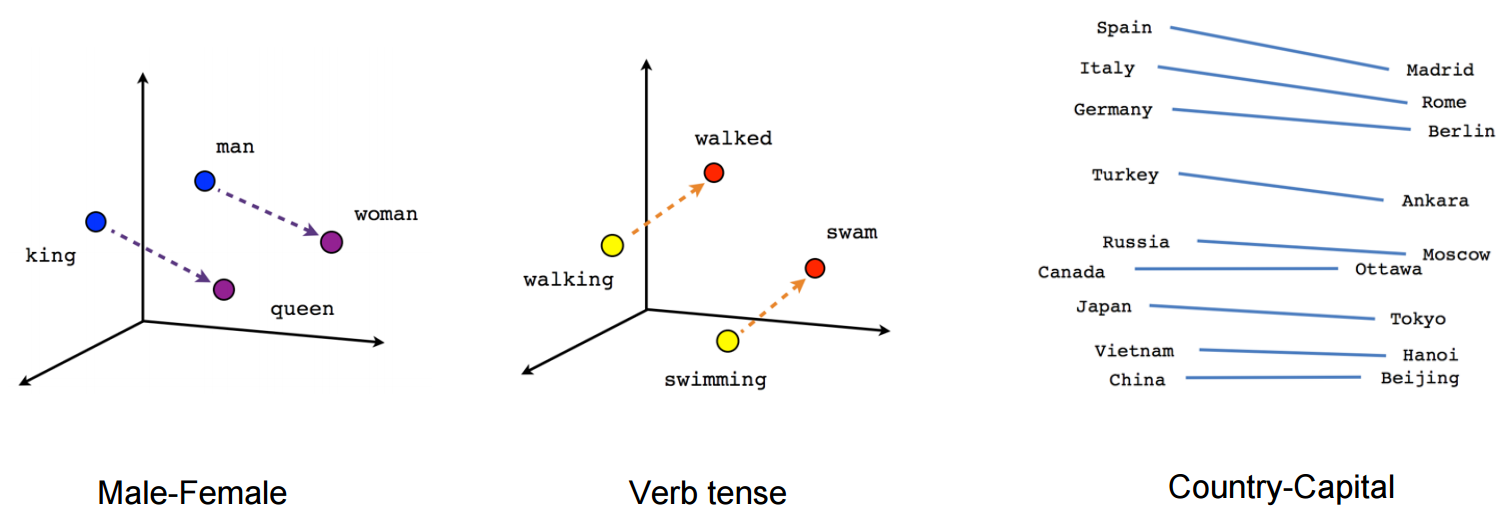
\includegraphics[width=0.8\linewidth]{linear-relationships}
\caption[Semantic regularities in distributed word embeddings.]{Semantic regularities in Word2Vec word embeddings \cite{w2v:tensor_flow}.}
\label{fig:sem_rel}
\end{figure}

\begin{figure}[hbtp]
\centering
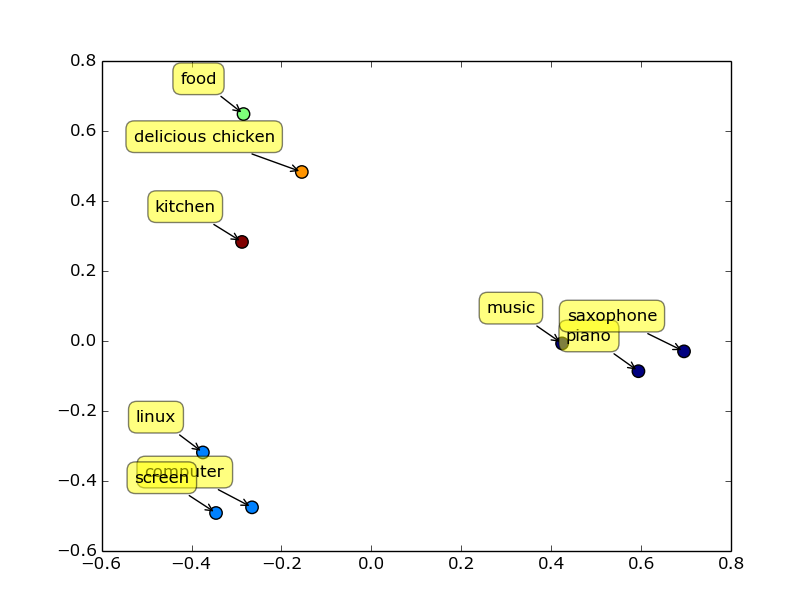
\includegraphics[width=0.8\linewidth]{word2vec_clustering}
\caption [Clustering of words in word embedding space.]{\textbf{Clustering of words in word embedding space: }{\small The figure shows the word clustering property of distributed word embeddings obtained by projecting the word vectors on two dimesional space using PCA. Figure adapted from: \text{https://github.com/aubry74/visual-word2vec}.}}
\label{fig:w2v_clustering}
\end{figure}

Another interesting property of distributed word embeddings is that the semantically related words are placed close to each other in a word embedding space \cite{w2v:mikolov_2013_distributed}, thus forming clusters of semantically related words (see fig. \ref{fig:w2v_clustering}). It was also observed that the word embeddings of similar words in different languages have the same geometrical arrangement in a word embedding space of respective language (see fig. \ref{fig:w2v_translation}). Therefore, it is also possible to learn the linear mapping between different word embedding space by vector rotation and scaling \cite{w2v:language_similarities}. Several other regularities can also be observed by performing the basic linear operation on word-embeddings \cite{w2v:mikolov_2013_distributed}. 

\begin{figure}[hbtp]
\centering
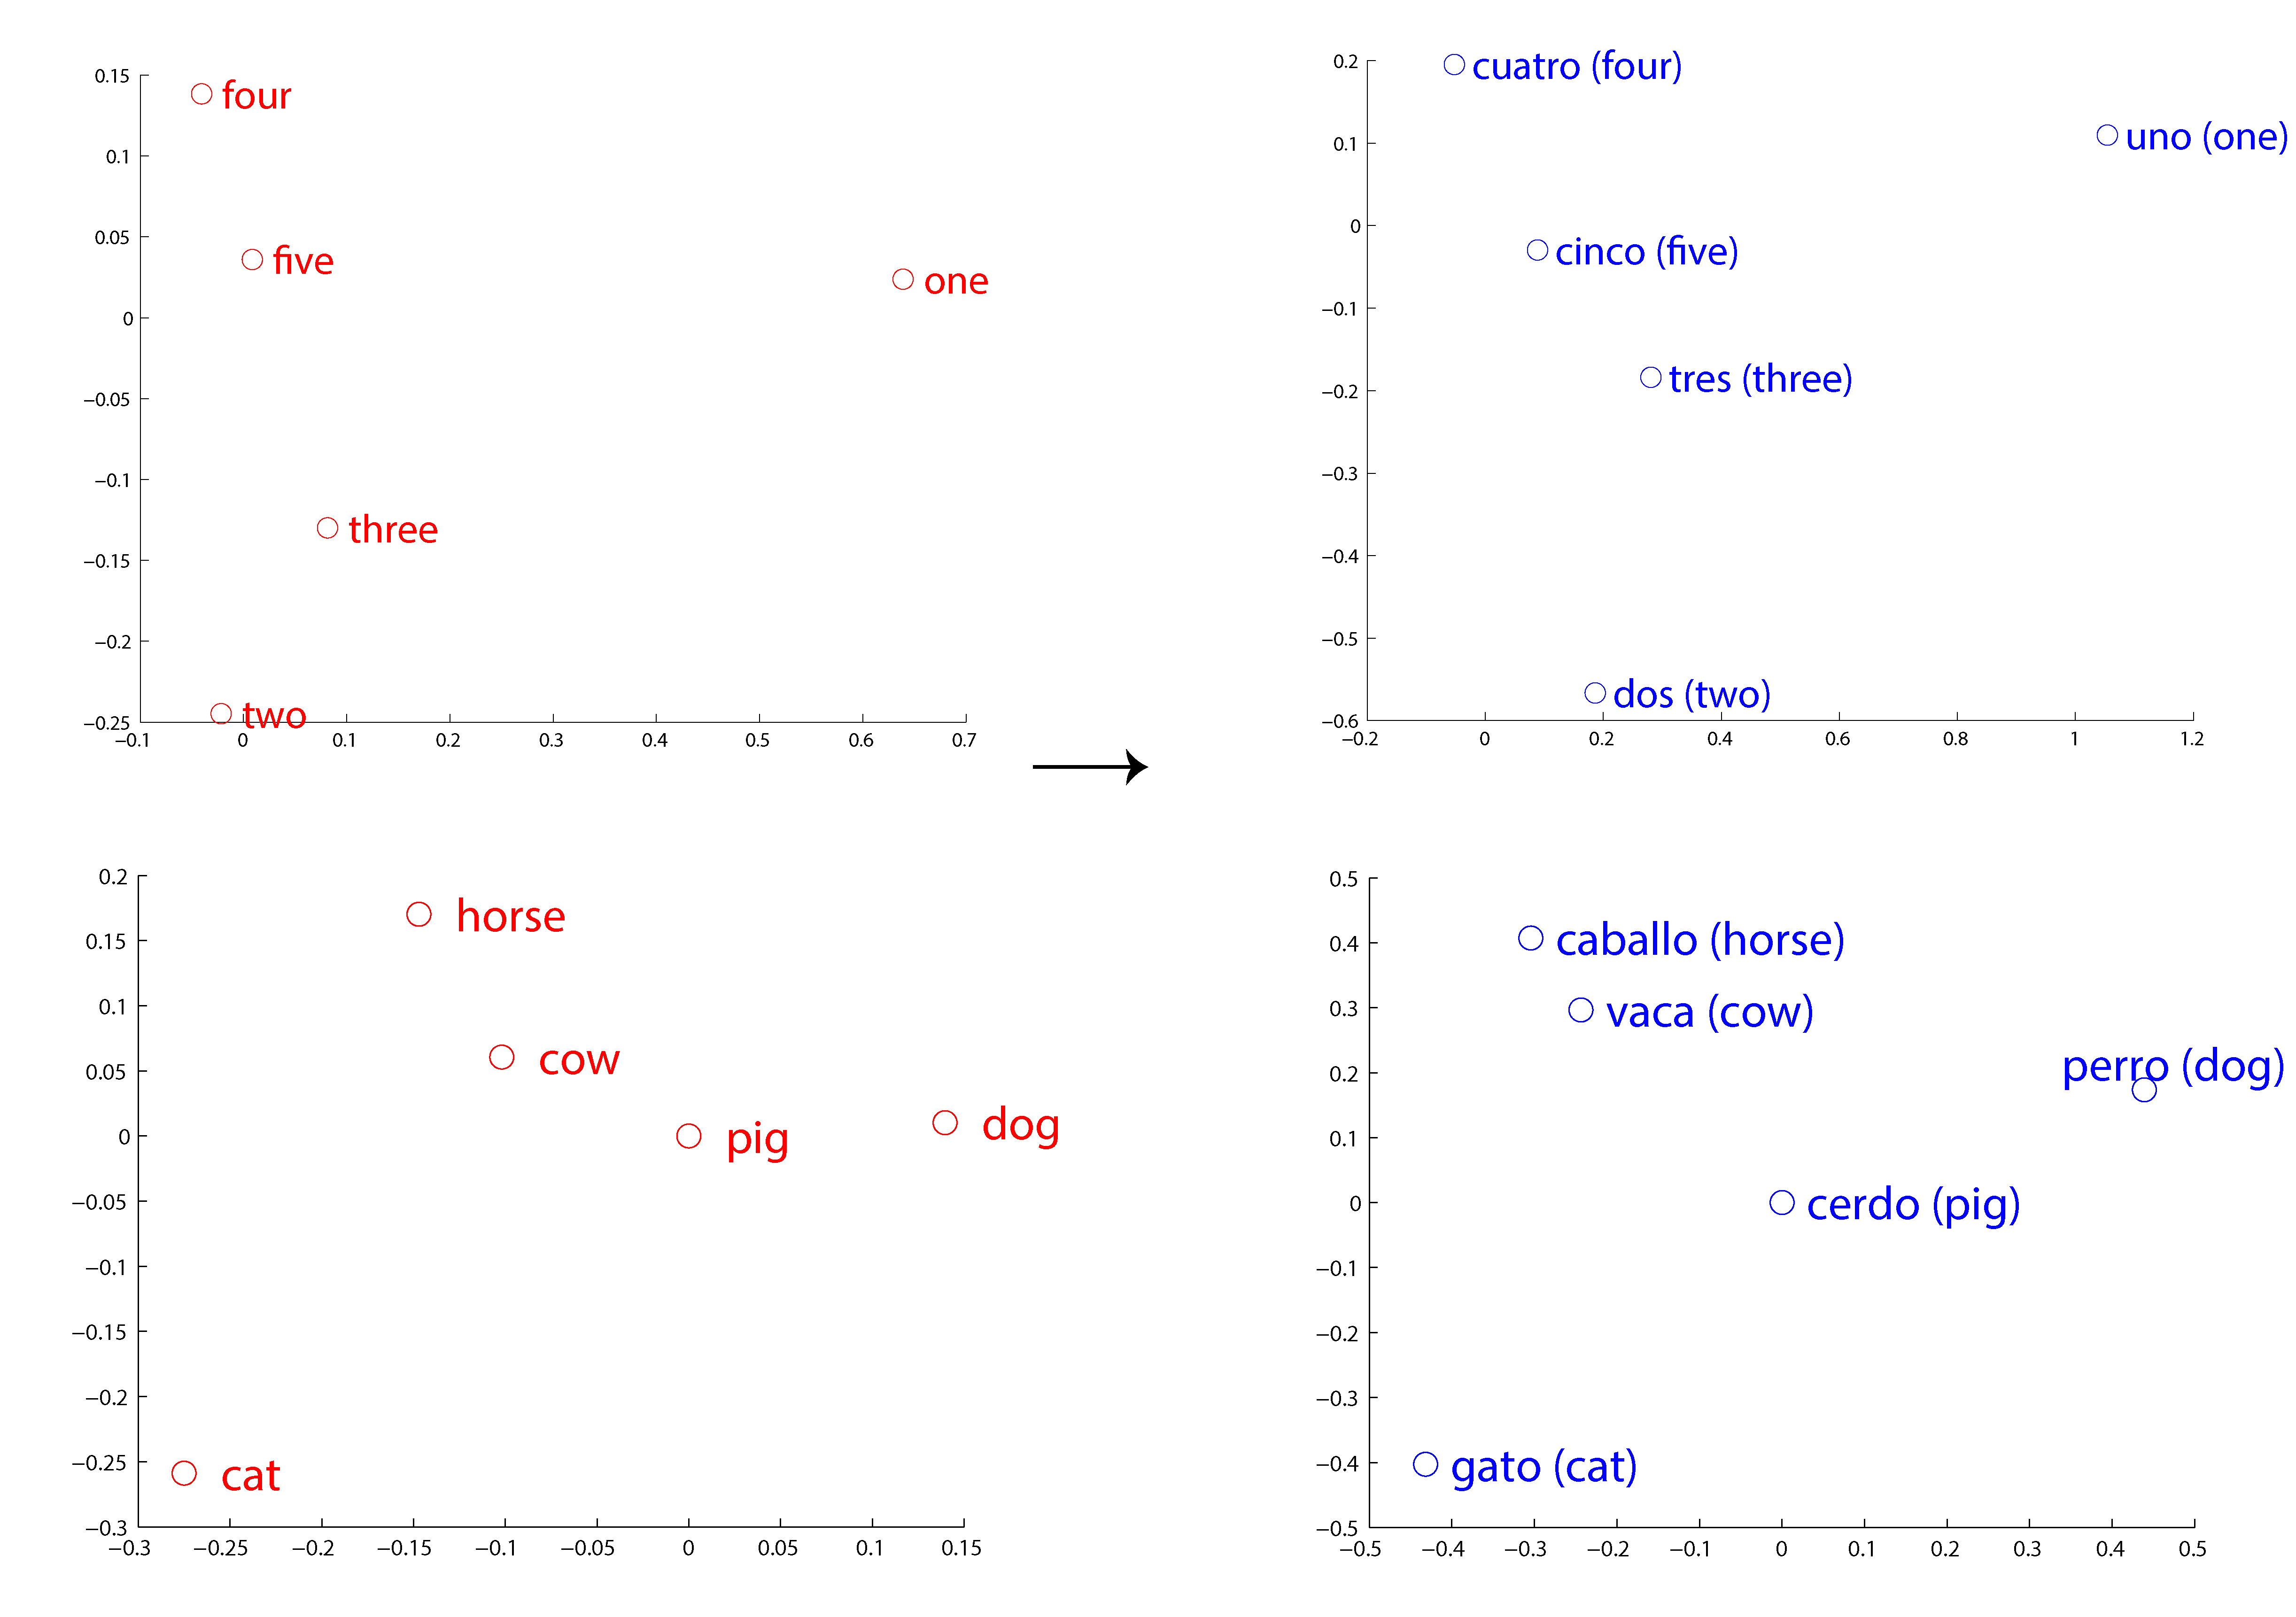
\includegraphics[width=0.8\linewidth]{word2vec_translation}
\caption[Language Translation property of distributed word vectors.]{\textbf{Language Translation property of distributed word vectors: }{\small The figure shows the distributed word vectors in English (left) and Spanish (right), projected in 2-D space using PCA. Notice that both the languages have the same geometrical arrangement of similar words in word embedding space. Thus, the word vectors in the English language can be rotated and scaled to obtain the word embeddings of similar words in Spanish. Figure adapted from \cite{w2v:language_similarities}.}}
\label{fig:w2v_translation}
\end{figure}

\section{Echo State Network (ESN)}

Echo State Network (ESN) is a network with a new viewpoint on Recurrent Neural Network (RNN). It is a discrete time continuous state recurrent neural network introduced by Jaeger \cite{esn:jaeger:2001} and is believed to resemble the learning mechanism in biological brains closely. ESN is found to be computationally simple and inexpensive to process the temporal or sequential data. The main idea of ESN is to operate a random, large, and crucially, fixed RNN with the input signal. The non-linear response generated by each neuron of the RNN is then collectively combined with the desired output signal using regression to learn the output weights \cite{esn:jaeger_tutorial, esn:jaeger:2001,esn:scholarpedia:2007}. It is worth noting that the ESN are not trained using error Back Propagation (BP) \cite{back_propagation} but, instead the linear regression is used. The reason for this choice is that the use of BP makes the training of RNN non-converging, slow, and computationally expensive \cite{bp_in_rnn}. Whereas, the training using linear regression is faster and computationally inexpensive \cite{esn:practical_guide}.  

\subsection{ESN Architecture}

\begin{figure}[hbtp]
\centering
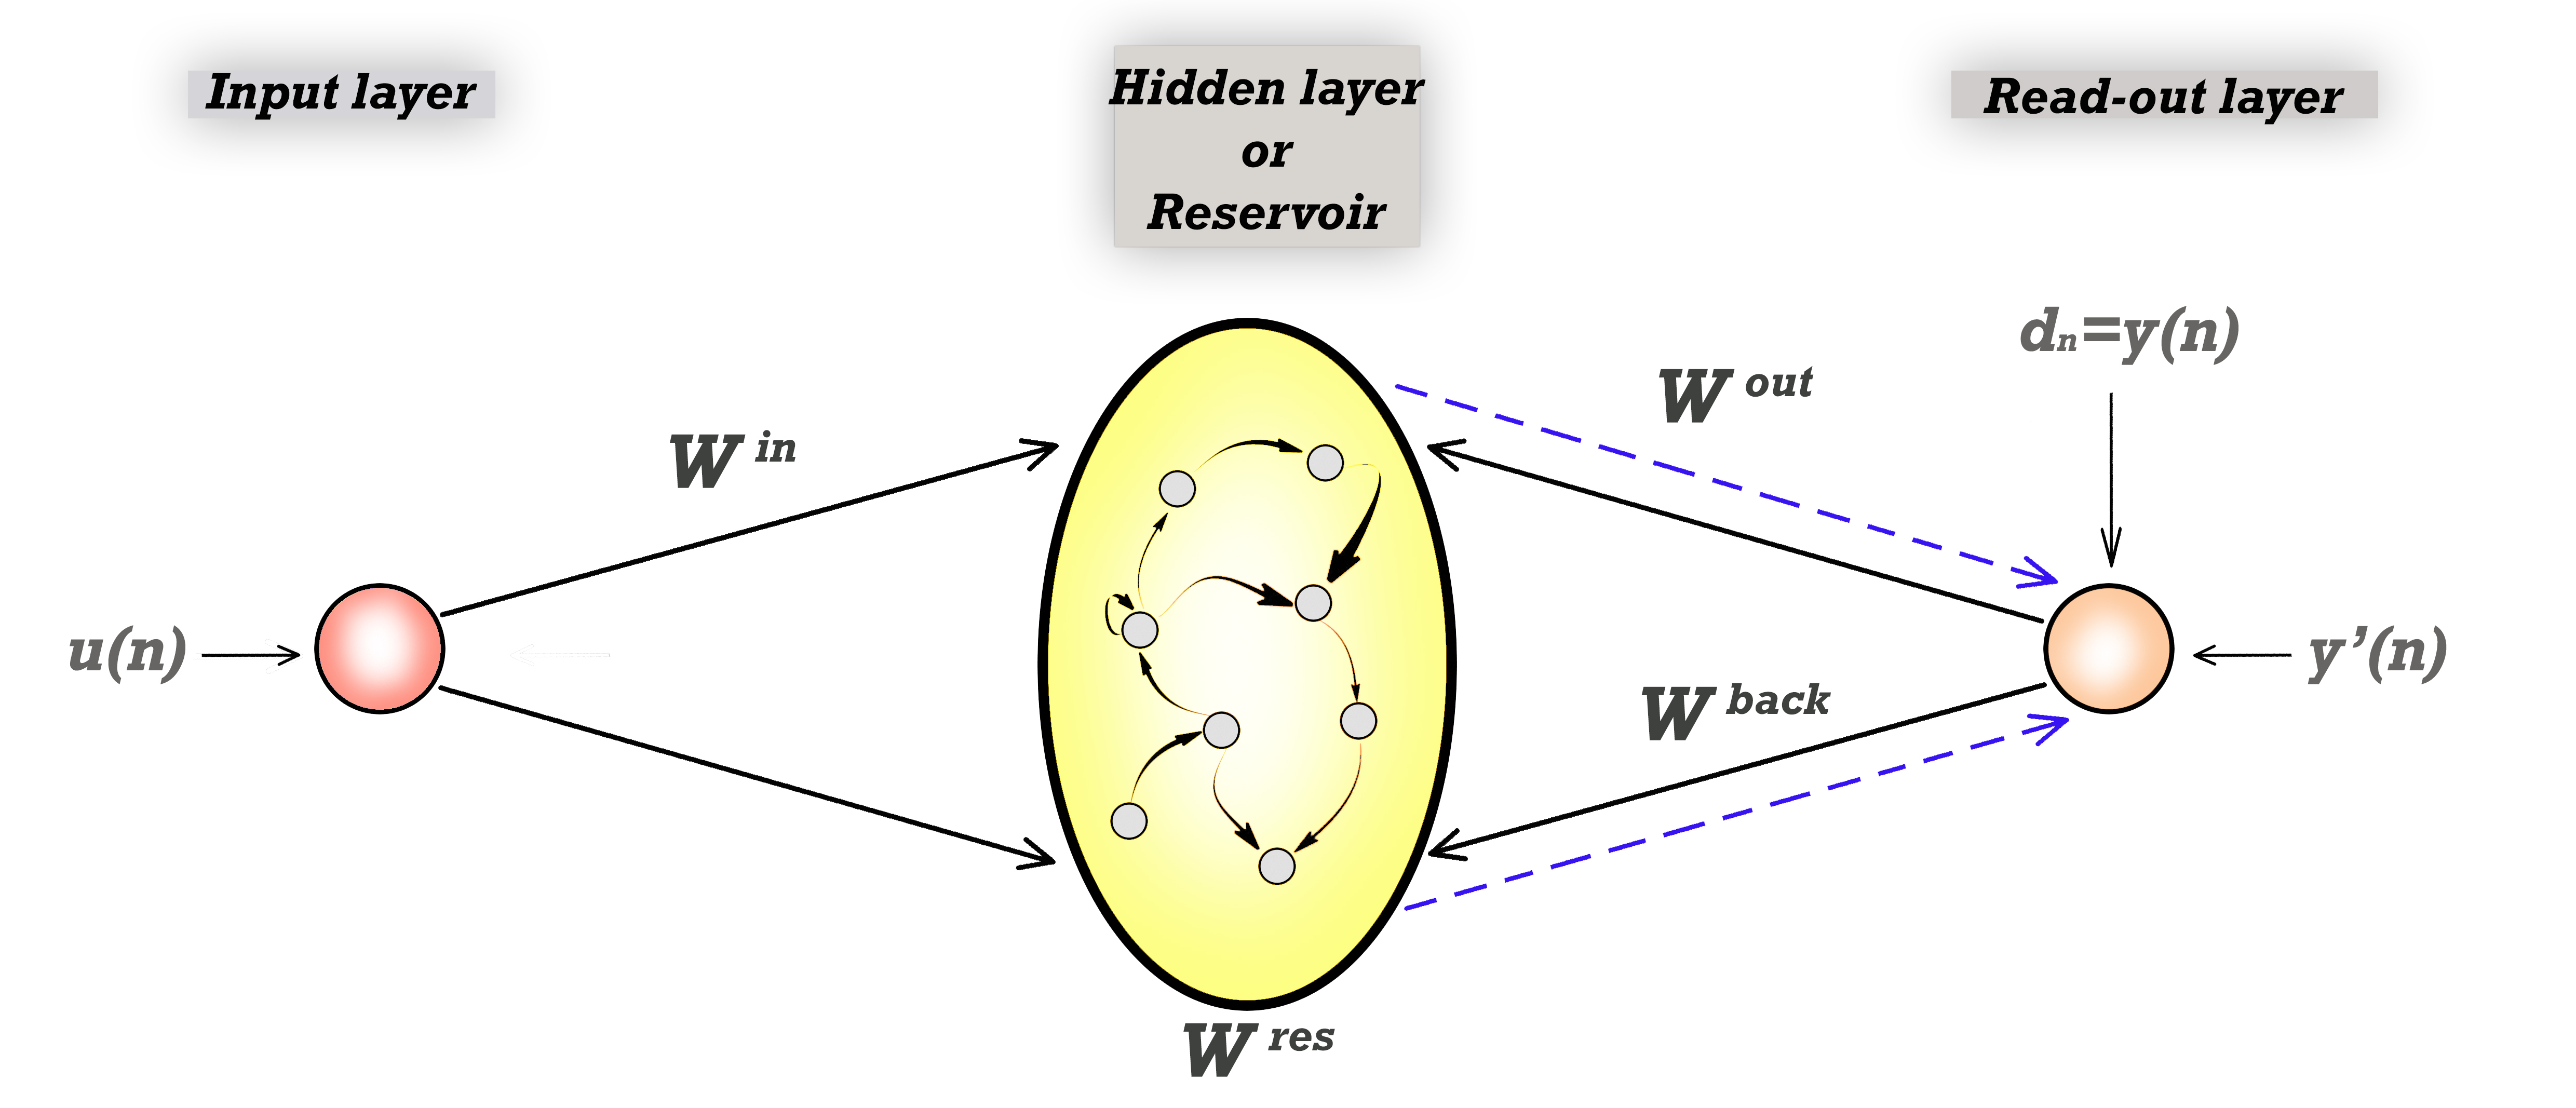
\includegraphics[width=0.8\linewidth]{esn_architecture}
\caption[Architecture of classical ESN.]{\textbf{Architecture of classical ESN: }{\small The reservoir is the recurrent neural network with $N_{x}$ neurons and randomly initialized connections. The reservoir is provided with an input sequence $u(n)$ from the input layer and the teacher signal $y(n)$ from the output layer during training. The input-to-reservoir weights ($W^{in}$), output-to-reservoir weights ($W^{back}$), and reservoir-to-reservoir weight ($W^{res}$) are randomly initialized and remain static during learning. The output weights from the reservoir to output units ($W^{out}$) are the only weights learned by the network during training. Adapted from \cite{esn:practical_guide}}}
\label{fig:esn_arch}
\end{figure}

ESN is a surprisingly efficient variant for training the RNNs. Figure \ref{fig:esn_arch} shows the basic architecture of an ESN. In a standard RNN, all the weights are required to be tuned, even though it was shown that RNN works well enough without full adaptation of weights \cite{esn:practical_guide}. The classical ESN mainly contains three layers, input layer, the hidden layer (also known as the reservoir) and the readout layer. The input layer is fully connected to the hidden layer, and both the hidden layer and the input layer are connected to the output layer. The output layer is fully connected back to the hidden layer. However, the connections from input-to-output and output-to-hidden layer are optional and depend on the task.

The weights from input-to-reservoir (i.e. $W^{in}$) and reservoir-to-reservoir (i.e. $W^{res}$) are sparsely (i.e. most of the elements in these matrices will be zero) and randomly initialized. The sparsity of $W^{in}$ and $W^{res}$ is however not a necessary condition but Jaeger \cite{esn:jaeger:2001} recommended the sparse initialization of these weights often give better performance. The non-zero element in the sparse input weight matrix $W^{in}$, and the reservoir weight matrix $W^{res}$, are usually generated from a uniform or normal distribution. The output-to-reservoir weights ($W^{back}$) are also randomly initialized. $W^{in}$, $W^{res}$ and $W^{back}$ weights remains untrained during the training whereas the weights from the reservoir-to-output layer (i.e. $W^{out}$) are the only weights learned during the supervised training \cite{esn:jaeger:2001, esn:practical_guide}. For the ESN approach to work, the reservoir should possess the \textit{Echo State Property (ESP)}: if a long input sequence is given to the reservoir the reservoir will end up in the same state irrespective of the initial reservoir state. In other words, the reservoir states `echoes' the input sequence and the effect of previous reservoir state and the previous input on the future reservoir states should vanish gradually \cite{esn:practical_guide, esn:jaeger_tutorial}. 

To ensure the echo state property in ESN, firstly, the reservoir weights matrix $W^{res}$ and the input weights matrix $W^{in}$ are often generated sparsely (not necessarily) and randomly from a normal or uniform distribution \cite{esn:practical_guide}. The input weight matrix is, however, a bit denser than the reservoir weight matrix. The sparsely generated random reservoir weight matrix $W^{res}$ is often scaled such that its spectral radius, $\rho(W^{res})$, i.e. largest absolute eigenvalue, is less than one \cite{esn:scholarpedia:2007}. However $\rho(W^{res}) < 1 $ is not a necessary condition for ESN to have the ESP and can be achieved even when $\rho(W^{res}) > 1$ \cite{esn:jaeger:2001, esn:practical_guide, esn:jaeger_tutorial}. Intuitively, the spectral radius is a crude measure of the amount of memory the reservoir can hold. The smaller values are used when short memory is required, and the larger values for a longer memory\cite{esn:practical_guide}.

To scale the randomly generated $W^{res}$ matrix, it is first divided by its spectral radius and then multiplied with the desired spectral radius \cite{esn:jaeger_tutorial}.

\begin{equation}\label{eqn:res_scaling}
W_{new}^{{res}}=\gamma \frac{W^{res}}{\rho(W^{res})}
\end{equation}

\noindent where $W_{_{new}}^{{res}}$ is the scaled reservoir weight matrix, $ \gamma$ is the desired spectral radius and $\rho(W^{res})$ is the spectral radius of the randomly generated reservoir matrix $W^{res}$.

The input weights ($W^{in}$) are also scaled to regulate the non-linearity in reservoir activations. A very high input scaling let the reservoir behave in a highly non-linear manner (because of the \textit{`tanh'} activation function) whereas a very small input scaling is used wherever linearity is required in a task \cite{esn:practical_guide}.

\subsection{Training ESN}\label{ssec:esn_training}

ESNs are mostly applied for supervised machine-learning tasks where the temporal or sequential aspect of the data is to be modeled. Before training, the reservoir of size $N_{x}$, generally containing leaky-integrated discrete-time continuous-value neurons with \textit{tanh} activation function are generated. The reservoir of any computationally affordable size can be used. The bigger the reservoir size, the more the input signal gets non-linearly expanded and easier it will be to find the linear combination with the desired output signal \cite{esn:practical_guide, esn:jaeger_tutorial}. The bigger reservoir size is however not always the best choice. With the big reservoir size comes the risk of over-fitting. Thus, it is also important to use proper regularization methods to avoid over-fitting. After generating the reservoir, the reservoir weights, $W^{res}$, the input weights, $W^{in}$, and the feedback weights, $W^{back}$, are randomly initialized.

The training objective of the ESN approach is to learn a model which outputs \textit{$y'$}, such that it is as close as possible to the target output \textit{y} by minimizing the some error measure, $E(y',y)$. The learned model should also be able to generalize well on the data not used for training. Root Mean Square Error (RMSE) is typically chosen as an error measure $E$. Thus during training, the given input signal $\textit{u(n)} \in \mathbb{R}^{N_u}$ and the corresponding teacher signal $\textit{y(n)} \in \mathbb{R}^{N_y}$  are input to the reservoir at every time-step `n'. Here n = 1, 2..., T is the discrete time step for sequence of length T. The reservoir then generates a sequence $\textit{x(n)} \in \mathbb{R}^{N_{x}}$ reservoir states which is a non-linear high dimensional expansion of the input signal $\textit{u(n)}$ \cite{esn:jaeger_tutorial}. The reservoir activation and reservoir state update is computed using following recursive equations:

\begin{equation} \label{eqn:res_update}
x'(n) =\textit {tanh } ( W^{res}x(n-1) + W^{in}.u(n) + W^{back}.y(n-1))
\end{equation}
\begin{equation} \label{eqn:res_state}
x(n) =\textit (1-\alpha) x(n-1) + \alpha x'(n)
\end{equation}

\noindent where $\textit{ x(n)}$ is the vector of reservoir neuron's activations and \textit{ $x'(n)$} is its update at time step $\textit{n}$ and \textit{`tanh'} is the reservoir neuron activation function. $ W^{in} \in \mathbb{R}^{{N_x} \times{N_u}}$ and $ W^{res} \in \mathbb{R}^{{N_x} \times{N_x}} $ are input weights and reservoir weights matrices respectively. $ W^{back} \in \mathbb{R}^{{N_x} \times{N_y}} $ is the optional output-to-reservoir weights matrix \footnote{this weight matrix is optional and is task specific} and $\alpha \in (0,1]$ is the leaking rate of neurons.  

The leaking rate, $\alpha$, regulates the speed of reservoir state update in discrete time. A smaller value of $\alpha$ induces slow reservoir dynamics thus ensuring the long short-term memory in ESN \cite{esn:practical_guide, esn:optimization_leaky_neurons}. The reservoir activation states are accumulated at every time step for regression with the teacher output. The linear readout weights are then learned using equations:

\begin{equation}\label{eqn:esn_output}
y'(n) = \textit W^{out}x(n)
\end{equation}

\noindent where $y'(n) \in \mathbb{R}^{N_y}$ is the output of the network and $W^{out} \in \mathbb{R}^{{N_y} \times {N_x}}$ is the output weight matrix.

Writing the equation \ref{eqn:esn_output} in matrix form, the output weights $W^{out}$ are then learned using the following equation:
 
\begin{equation}
Y'=W^{out}X
\end{equation}
\begin{equation}
W^{out}=Y'X^{T}(XX^{T}+{\beta}I)^{-1}
\end{equation}

\noindent where $\beta$ is the regularization coefficient parameter of ridge regression and \textit{I} is the Identity matrix. 

Training procedure of ESN has only a few global parameters which are to be optimized: the reservoir size $ N_{x} $, spectral radius of $W^{res}$, input scaling of $W^{in}$, leak rate $\alpha$ and the ridge parameter $\beta$. All these parameters can only be optimized by trial and error method and depend heavily on the task under consideration \cite{esn:practical_guide}. Usually, a grid search is applied to explore the best parameter combination. 